%! Author = Omar Iskandarani
%! Title = Standaardmodel-Lagrangian in Vortex Æther Model-Eenheden
%! Date = May 23, 2025
%! Affiliation = Independent Researcher, Groningen, The Netherlands
%! License = CC-BY 4.0
%! ORCID = 0009-0006-1686-3961

\documentclass[a4paper, aps,preprint,superscriptaddress, 12pt]{revtex4}
\usepackage[a4paper, margin=2cm]{geometry}
\usepackage{bookmark}
\usepackage{float}
\usepackage{tikz}
\usepackage{makecell}
\usepackage{tabularx}
\usepackage[font=footnotesize]{caption}
\usetikzlibrary{arrows.meta}
\usepackage{pgfplots}
\pgfplotsset{compat=1.18}
\usepackage[none]{hyphenat}
\usepackage{array}
\usepackage{amsmath}
\usepackage{booktabs}
\usepackage[utf8]{inputenc}
\usepackage{amssymb}
\usepackage{graphicx}
\usepackage{hyperref}
\usepackage{physics}
\usepackage{natbib}
\usepackage{url}
\usepackage{multirow}
\usepackage{subcaption}
\usepackage{siunitx}
\usepackage{listings}
\renewcommand{\arraystretch}{1.5}
\renewcommand{\floatpagefraction}{.8}
\sloppy

\begin{document}

\author{Omar Iskandarani}
\title{Standaardmodel-Lagrangian in Vortex Æther Model-Eenheden}
\date{Mei 2025}
\affiliation{Independent Researcher, Groningen, The Netherlands}
\thanks{ORCID: \href{https://orcid.org/0009-0006-1686-3961}{0009-0006-1686-3961}}
\email{info@omariskandarani.com}

\begin{abstract}
We present a reformulation of the Standard Model Lagrangian using the dimensional and topological framework of the Vortex Æther Model (VAM). In this formulation, conventional quantum field terms are reinterpreted through fluid-mechanical analogs, where particles correspond to knotted vortex excitations in a compressible æther, and interactions arise from swirl, circulation, and density fluctuations. A complete set of natural units replaces Planck-based constants, rooted in mechanical quantities such as core radius (\(r_c\)), swirl velocity (\(C_e\)), and maximum æther force (\(F^\text{vam}_\text{max}\)). We demonstrate how gauge fields emerge from swirl dynamics, fermionic behavior from knotted helicity propagation, and mass generation from internal topological tension rather than spontaneous symmetry breaking. This reinterpretation leads to a dimensionally self-consistent Lagrangian, where all couplings and field dynamics are geometrically and physically grounded. The resulting model offers a unified mechanical ontology for quantum fields and suggests new avenues for interpreting mass, charge, and time from first principles.
\end{abstract}

    \maketitle

    % Canvas inputs
    %! Author = Omar Iskandarani
%! Date = 5/19/2025

\section{Inleiding en VAM-grondslagen}

Het Vortex Æther Model (VAM) beschouwt materie als stabiele vortexknopen (wervelknopen) in een alomtegenwoordig superfluïd æther~\cite{Kelvin1867VortexAtoms}. Belangrijke parameters in VAM zijn de tangentiële kernrotatiesnelheid $C_e$, de vortexkernstraal $r_c$ en de
ætherdichtheid $\rho_{\ae}$, die op kernschaal vaste waarden aannemen (zie Tabel 1). Deze bepalen de kwantisering van circulatie en de maximale vortexkracht in het æthermedium. Een opmerkelijk uitgangspunt is dat vorticiteit (circulatie) behouden en gekwantiseerd is – analoog aan fluxkwantisatie – waardoor elke vortexknoop topologisch invariant (knopen kunnen niet continu ontwarren) en daarmee stabiel is. Dit biedt een mechanisme om massa en lading emergent te verklaren uit fluïdumwetten in plaats van via elementaire puntdeeltjes.

In VAM dragen vortexknopen heliciteit – de topologische koppeling van wervellijnen – die fungeert als interne vrijheidsgraad (vergelijkbaar met
spin) en ook geassocieerd wordt met lading. Heliciteit $H$ is gedefinieerd als de volumelijke integraal van de snelheid $v$ en vorticiteit $\omega$~\cite{Moffatt1990VortexHelicity, Ricca1992EnergyHelicity}:


\begin{equation}
    H = \int \mathbf{v} \cdot \boldsymbol{\omega}\,dV,
\end{equation}

een behouden grootheid die de linking/winding van wervelstructuren telbaar maakt. Intuïtief telt $H$ het (gekwantiseerde) aantal omwentelingen waarmee wervel-lijnen elkaar omcirkelen. Deze topologische invariantie ($H$ constant) garandeert dat een gesloten vortexknoop een minimale energieconfiguratie niet spontaan kan verliezen zonder externe inwerking.

Tabel 1 hieronder resumeert enkele fundamentele VAM-constanten voor het kernschaal-regime:

\begin{table}[h!]
    \centering
    \begin{tabular}{lll}
        \hline
        Symbool & Grootheid & Waarde (kernscala)\\
        \hline
        $C_e$ & Tangentiële kernrotatiesnelheid & $1.094\times10^6~\text{m/s}$\\
        $r_c$ & Vortexkernstraal (Coulomb-barrière straal) & $1.409\times10^{-15}~\text{m}$\\
        $\rho_{\ae}$ & Æther-dichtheid (lokaal) & $3.893\times10^{18}~\text{kg/m}^3$\\
        $F_{\max}$ & Maximale vortexkracht & $\approx 29~\text{N}$\\
        $\kappa$ & Circulatiekwantum ($C_e r_c$) & $1.54\times10^{-9}~\text{m}^2/\text{s}$\\
        $\alpha$ & Fijnstructuurconstante $(2C_e/c)$ & $7.297\times10^{-3}$\\
        \hline
    \end{tabular}
    \caption{Kernparameters in het Vortex Æther Model. Deze karakteristieke constanten bepalen de schaal van vortexkernen en interacties binnen nucleonen.}
\end{table}
    \section{Motivation}

The Standard Model Lagrangian is one of the most successful constructs in modern physics, unifying electromagnetic, weak, and strong interactions within a renormalizable quantum field theory. Yet it remains structurally incomplete in a physical sense: its mass terms, symmetry groups, and coupling constants are introduced \textit{a priori}, without geometric or mechanical derivation.

For instance, the fine-structure constant $\alpha \approx 1/137$ appears as an empirical ratio with no explanation for its value. The elementary charge $e$ and Planck constant $\hbar$ are similarly inserted into the theory to match experimental outcomes, but have no origin within the theory’s own framework. Even the Higgs vacuum expectation value (VEV), essential for mass generation, is externally imposed rather than derived.

The Vortex Æther Model (VAM) addresses these gaps by reconstructing the Standard Model from the ground up using topologically and mechanically grounded vortex structures. Rather than assuming discrete point particles and abstract quantum fields, VAM postulates a compressible, rotating æther medium in which all elementary particles are topologically stable vortex knots. Their observable properties—mass, charge, spin, and even local time—emerge from measurable fluidic parameters such as circulation strength, core radius, helicity, and swirl velocity.

In this framework, constants such as $\alpha$ and $\hbar$ are not arbitrary. For example, $\alpha$ is shown to emerge from the swirl geometry of the æther via the dimensionless ratio $\alpha = 2C_e / c$, while $\hbar$ is interpreted as a manifestation of quantized circulation within a vortex structure. These reconstructions offer not only physical intuition, but also potential explanations for why such constants take the values they do. A summary comparison is presented in Table~\ref{tab:SM_vs_VAM_constants}, contrasting key constants across both frameworks.

This approach aligns with principles established in superfluid dynamics, topological field theory, and analog gravity systems. By expressing Standard Model terms in VAM units and connecting abstract constants to physical flow properties, the model opens pathways to new testable predictions—particularly regarding vacuum energy, neutrino mass generation, and mechanisms of quark confinement.



\subsection*{Unified Constants and Units in VAM}

The table below summarizes the complete set of mechanical and topological quantities used throughout the Vortex Æther Model. These values form a self-contained replacement for Planck-based dimensional analysis.


\begin{table}[H]
    \centering
    \footnotesize
    \renewcommand{\arraystretch}{1.3}
    \begin{tabular}{|l|l|l|l|}
        \hline
        \textbf{Symbol} & \textbf{Formula / Definition} & \textbf{Interpretation in VAM} & \textbf{Approx. Value (SI)} \\
        \hline

        $C_e$ &
        — &
        Core swirl velocity; sets intrinsic time rate of particles &
        $1.094 \times 10^6$ m/s \\
        \hline

        $r_c$ &
        — &
        Radius of vortex core; spatial extent of a particle &
        $1.409 \times 10^{-15}$ m \\
        \hline

        $\rho_\text{\ae}$ &
        — &
        Æther density; determines flow inertia and stress limits &
        $3.893 \times 10^{18}$ kg/m³ \\
        \hline

        $F^{\text{vam}}_\text{max}$ &
        $\pi r_c^2 C_e \rho_\text{\ae}$ &
        Max transmissible force through æther (vortex core tension) &
        $\sim 29.05$ N \\
        \hline

        $F^{\text{gr}}_\text{max}$ &
        $\frac{c^4}{4G}$ &
        GR-based theoretical maximum force limit &
        $\sim 3.0 \times 10^{43}$ N \\
        \hline

        $\kappa$ &
        $\frac{\Gamma}{n}$ or quantized $\oint \vec{v} \cdot d\vec{\ell}$ &
        Quantum of circulation per vortex loop &
        $1.54 \times 10^{-9}$ m²/s \\
        \hline

        $\alpha$ &
        $\frac{2 C_e}{c}$ &
        Fine-structure constant from swirl-to-light ratio &
        $7.297 \times 10^{-3}$ (unitless) \\
        \hline

        $t_P$ &
        $\frac{r_c}{c}$ &
        Fastest rotation cycle (Planck time analog) &
        $\sim 5.39 \times 10^{-44}$ s \\
        \hline

        $\Gamma$ &
        $\oint \vec{v} \cdot d\vec{\ell}$ &
        Total circulation; encodes angular momentum &
        (typical unit: m²/s) \\
        \hline

        $t$ &
        $dt \propto \frac{1}{\vec{v} \cdot \vec{\omega}}$ &
        Local time rate derived from helicity field configuration &
        (unit: s) \\
        \hline

        $\mathcal{H}_\text{topo}$ &
        $\int \vec{v} \cdot \vec{\omega} \, dV$ &
        Topological helicity; measures vortex alignment &
        (unit: m³/s²) \\
        \hline
    \end{tabular}
    \caption{Fundamental parameters in the Vortex Æther Model (VAM). These quantities form the physical and topological basis for mass, time, charge, and quantum behavior. Each is experimentally meaningful and derivable from ætheric flow geometry.}
    \label{tab:VAM_master_table}
\end{table}


\subsection*{Derived Couplings and Constants in VAM}
From the core æther parameters introduced above, several familiar physical constants can be re-expressed as derived quantities. These include the Planck constant, the speed of light, the fine-structure constant, and the elementary charge—all reconstructed as emergent properties of swirl and circulation. Table~\ref{tab:VAM_master_table} summarizes these reformulations.

Within VAM, the maximum vortex interaction force is derived explicitly from Planck-scale physics:
\begin{equation}
    F^{\text{vam}}_\text{max} = \alpha \left(\frac{c^4}{4G}\right)  \left(\frac{r_c}{l_p}\right)^{-2}
\end{equation}

where $\frac{c^4}{4G}$ is the Maximum Force in nature $F^{\text{gr}}_\text{max}$, the stress limit of the æther found from General Relativity, and $l_p$ is the Planck Length.


\subsection*{Comparative Origins of Constants: Standard Model vs. VAM}

The re-expression of fundamental constants within VAM highlights a key philosophical and physical distinction: while the Standard Model treats quantities like $\alpha$, $\hbar$, and $e$ as empirical inputs, the Vortex Æther Model derives them from topological and geometric features of the æther flow.

The table below contrasts how key constants are introduced or derived in both frameworks.

\begin{table}[H]
    \centering
    \footnotesize
    \renewcommand{\arraystretch}{1.3}
    \begin{tabular}{|l|l|l|}
        \hline
        \textbf{Constant} & \textbf{Standard Model Treatment} & \textbf{VAM Derivation / Interpretation} \\
        \hline
        \makecell[l]{Fine-Structure \\ Constant $\alpha$} &
        \makecell[l]{Empirical dimensionless constant \\ for EM interaction strength} &
        \makecell[l]{Emerges from swirl ratio: \\ $\alpha = \frac{2 C_e}{c}$; purely geometric} \\
        \hline

        \makecell[l]{Planck Constant \\ $\hbar$} &
        \makecell[l]{Postulated quantum of action; \\ enters commutation rules} &
        \makecell[l]{Circulation-induced impulse: \\ $\hbar \sim \rho_\text{\ae} \Gamma r_c^2$} \\
        \hline

        \makecell[l]{Elementary \\ Charge $e$} &
        \makecell[l]{Input coupling in QED \\ with no internal structure} &
        \makecell[l]{Swirl flux through vortex core: \\ $e \sim \rho_\text{\ae} C_e r_c^2$} \\
        \hline

        \makecell[l]{Speed of \\ Light $c$} &
        \makecell[l]{Postulated invariant limit \\ in SR and GR} &
        \makecell[l]{Calibration limit; \\ signal speed is $C_e < c$ \\ (Lorentz symmetry is emergent)} \\
        \hline

        \makecell[l]{Higgs VEV \\ $v$} &
        \makecell[l]{Free symmetry-breaking scale; \\ not derived internally} &
        \makecell[l]{Ætheric tension amplitude: \\ $v \sim \sqrt{F_\text{max}/\rho_\text{\ae}}$} \\
        \hline

        \makecell[l]{Maximum \\ Force $F_\text{max}$} &
        \makecell[l]{Rare in SM; from GR: \\ $F = c^4/4G$ in limit cases} &
        \makecell[l]{Derived from vortex tension: \\ $F_\text{max}^{\text{vam}} = \pi r_c^2 C_e \rho_\text{\ae}$} \\
        \hline
    \end{tabular}
    \caption{Ontological contrast between the Standard Model and the Vortex Æther Model regarding the origin of key physical constants. VAM replaces empirical insertions with mechanical derivations from swirl and æther geometry.}
    \label{tab:SM_vs_VAM_constants}
\end{table}

\section*{Foundational Contrasts: Constants and Particles in VAM vs. SM}

Beyond constants, the Standard Model also posits intrinsic properties of particles—mass, spin, charge, flavor—as axiomatic features of quantized fields. The Vortex Æther Model, by contrast, interprets these as emergent from topological and dynamic features of vortex structures in a rotating æther medium.
\begin{table}[H]
    \centering
    \footnotesize
    \renewcommand{\arraystretch}{1.3}
    \begin{tabular}{|l|l|l|}
        \hline
        \textbf{Particle Property} & \textbf{Standard Model Interpretation} & \textbf{VAM Interpretation} \\
        \hline
        \makecell[l]{Mass} &
        \makecell[l]{Introduced via Higgs field \\ with arbitrary Yukawa couplings} &
        \makecell[l]{Emergent from vortex inertia: \\ $m \propto \rho_\text{\ae} \Gamma / C_e$ \\ or tension within knotted core} \\
        \hline
        \makecell[l]{Spin} &
        \makecell[l]{Intrinsic angular momentum \\ ($\hbar/2$ for fermions)} &
        \makecell[l]{Topological twist of vortex core \\ (e.g., Möbius loop linking)} \\
        \hline
        \makecell[l]{Electric Charge} &
        \makecell[l]{Coupling to $U(1)$ gauge field; \\ conserved via symmetry} &
        \makecell[l]{Swirl flux through core: \\ $e \sim \rho_\text{\ae} C_e r_c^2$ \\ (sign from swirl handedness)} \\
        \hline
        \makecell[l]{Flavor (Generations)} &
        \makecell[l]{Empirically distinct; \\ no structural rationale} &
        \makecell[l]{Knot complexity or higher-order \\ toroidal mode excitations} \\
        \hline
        \makecell[l]{Color Charge} &
        \makecell[l]{$SU(3)$ triplet charges; \\ source of strong force} &
        \makecell[l]{Filament braiding states or \\ phase twist between vortices} \\
        \hline
        \makecell[l]{Antiparticles} &
        \makecell[l]{Charge-conjugated fields \\ with opposite quantum numbers} &
        \makecell[l]{Mirror vortices with opposite \\ helicity and circulation} \\
        \hline
        \makecell[l]{Mixing (CKM/PMNS)} &
        \makecell[l]{Unitary matrices for \\ mass eigenstate mixing} &
        \makecell[l]{Oscillations from vortex coupling \\ or internal torsion precession} \\
        \hline
    \end{tabular}
    \caption{Ontological contrast between the Standard Model and the Vortex Æther Model in explaining intrinsic particle properties. In VAM, each feature arises from topological structure and flow dynamics within the æther.}
    \label{tab:SM_vs_VAM_particles}
\end{table}




    \input{03_natural_æther_constants}
    \section{Reformulating the Standard Model Lagrangian in VAM Units}\label{sec:lagrangian_vam}
The Standard Model Lagrangian encapsulates particle dynamics through symmetry-based field terms:
\begin{equation}
    \mathcal{L}_{\text{SM}} = -\frac{1}{4}F^{\mu\nu}F_{\mu\nu} + i\bar{\psi}\gamma^\mu D_\mu \psi + y_f \bar{\psi}\phi \psi + |D_\mu \phi|^2 - V(\phi)
\end{equation}
While mathematically elegant, these terms are not derived from first physical principles but are inserted axiomatically. The Vortex Æther Model (VAM) replaces this abstraction with a Lagrangian based on vortex dynamics, æther strain, and helicity conservation.

\subsection*{Core Assumptions}
\begin{itemize}
    \item The æther is a compressible, barotropic superfluid with stable vortex excitations.
    \item Particles are topologically stable vortex knots with quantized circulation.
    \item The Euler–Lagrange formalism applies to the action integral over fluid kinetic and potential energy densities.
    \item Helicity and vorticity are conserved modulo reconnection events.
\end{itemize}

\subsection*{Remarks on Spacetime Treatment}

In this model, the action integral is expressed as:
\[
    S = \int dt \int_{\mathbb{R}^3} \mathcal{L}(\vec{v}, \Phi, \rho_\text{\ae}, \dots) \, d^3x,
\]
reflecting a 3+1 decomposition with \textbf{absolute Newtonian time} and \textbf{Euclidean spatial geometry}.

Unlike relativistic field theories defined on Minkowski space \( \mathbb{R}^{1,3} \), the VAM adopts a \textbf{non-relativistic ontology}, where time is globally ordered and external to field dynamics.

This approach is consistent with established non-relativistic field theories, such as the Gross–Pitaevskii and hydrodynamic models for Bose–Einstein condensates, where space and time are decoupled and the Lagrangian formalism operates over \( \mathbb{R}^3 \times \mathbb{R} \)~\cite{Pethick2008BEC}.

Relativistic invariance in this context is regarded as an \textbf{emergent symmetry} that may arise at large scales or in specific limits of vortex behavior.

\subsection*{VAM-Reformulated Lagrangian}
Each term in the SM Lagrangian maps to a mechanical analog:

\begin{align*}
    \mathcal{L}_\text{VAM} &= \underbrace{-\frac{1}{4} \sum_{a} W^{a}_{\mu\nu} W^{a\mu\nu}}_{\text{Gauge field vorticity}}
    + \underbrace{\sum_{f} i \, m_f C_e r_c \, \bar{\psi}_f \gamma^\mu D_\mu \psi_f}_{\text{Fermion swirl propagation}} \\
    &- \underbrace{|D_\mu \phi|^2}_{\text{Æther strain field}}
    - \underbrace{V(\phi)}_{\text{Æther compression potential}}
    - \underbrace{\sum_f y_f \bar{\psi}_f \phi \psi_f + \text{h.c.}}_{\text{Mass coupling}}
    + \underbrace{\mathcal{H}_\text{topo}}_{\text{Vortex helicity term}}
\end{align*}

Where:
\[
    V(\phi) = -\frac{F_\text{max}}{r_c}|\phi|^2 + \lambda |\phi|^4
    \quad \text{and} \quad \mathcal{H}_\text{topo} = \int \vec{v} \cdot \vec{\omega} \, dV
\]
The full variational derivation of this Lagrangian—including Euler–Lagrange equations for velocity, scalar, and density fields—is provided in Appendix~\ref{sec:EL-derivation}.

\subsection{Gauge Fields as Vorticity Structures}
From Helmholtz’s theorem, the energy density in a vortex field is:
\begin{equation}
    \mathcal{L}_{\text{swirl}} = \frac{1}{2} \rho_\text{\ae} \left( |\vec{v}|^2 + \lambda |\nabla \times \vec{v}|^2 \right)
\end{equation}
Here, $\vec{v}$ is swirl velocity; $\lambda$ captures æther compressibility. Incompressible flows correspond to pure gauge configurations ($\nabla \cdot \vec{v} = 0$), while compressible strains allow field strength analogs.

\begin{figure}[H]
    \centering
    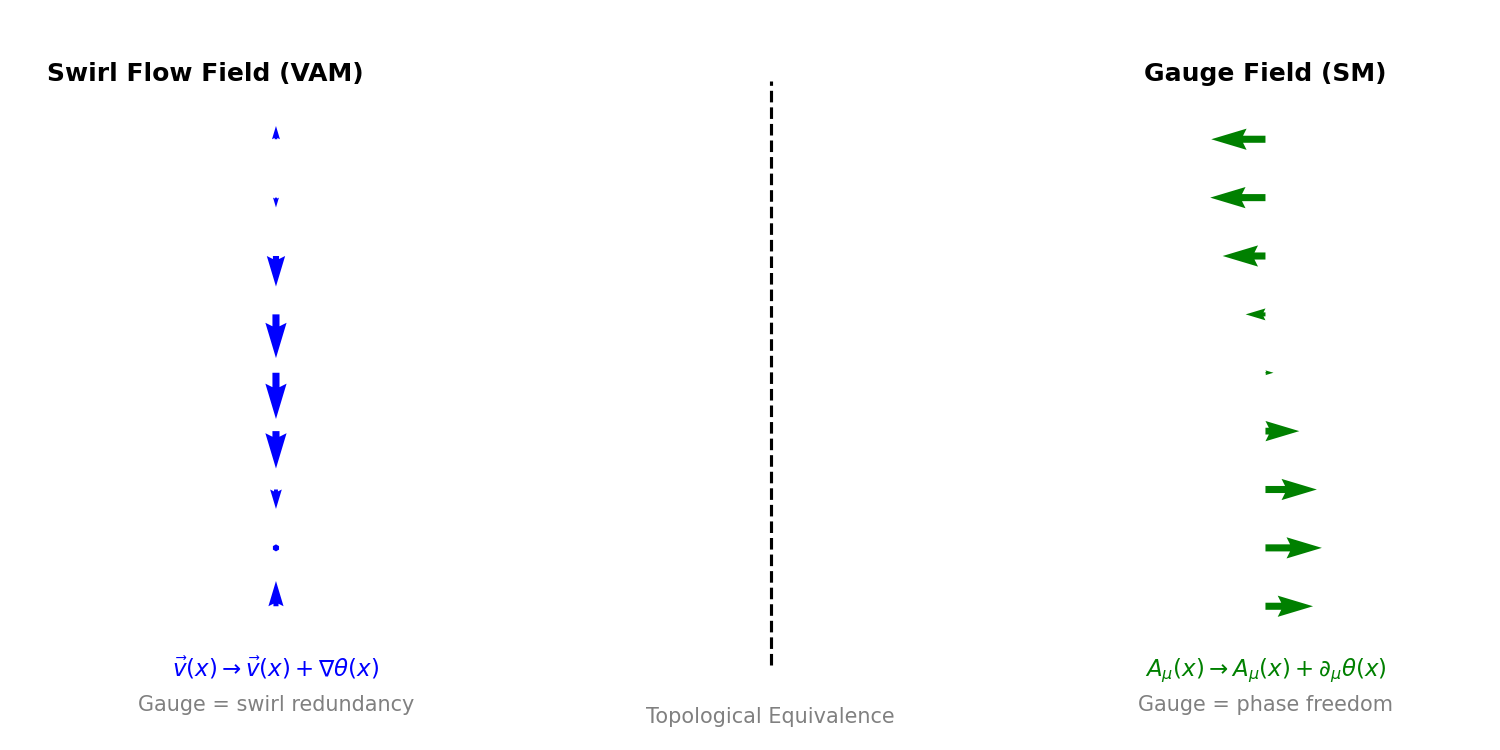
\includegraphics[width=0.95\textwidth]{gauge_swirl_equivalence}
    \caption{Analogy between gauge symmetry in the Standard Model and swirl invariance in the Vortex Æther Model (VAM). Both allow local reparameterizations that leave physical observables unchanged. Gauge symmetry in quantum field theory is structurally equivalent to potential-flow invariance in vortex dynamics.}
    \label{fig:gauge_swirl_equivalence}
\end{figure}

\begin{figure}[H]
    \centering
    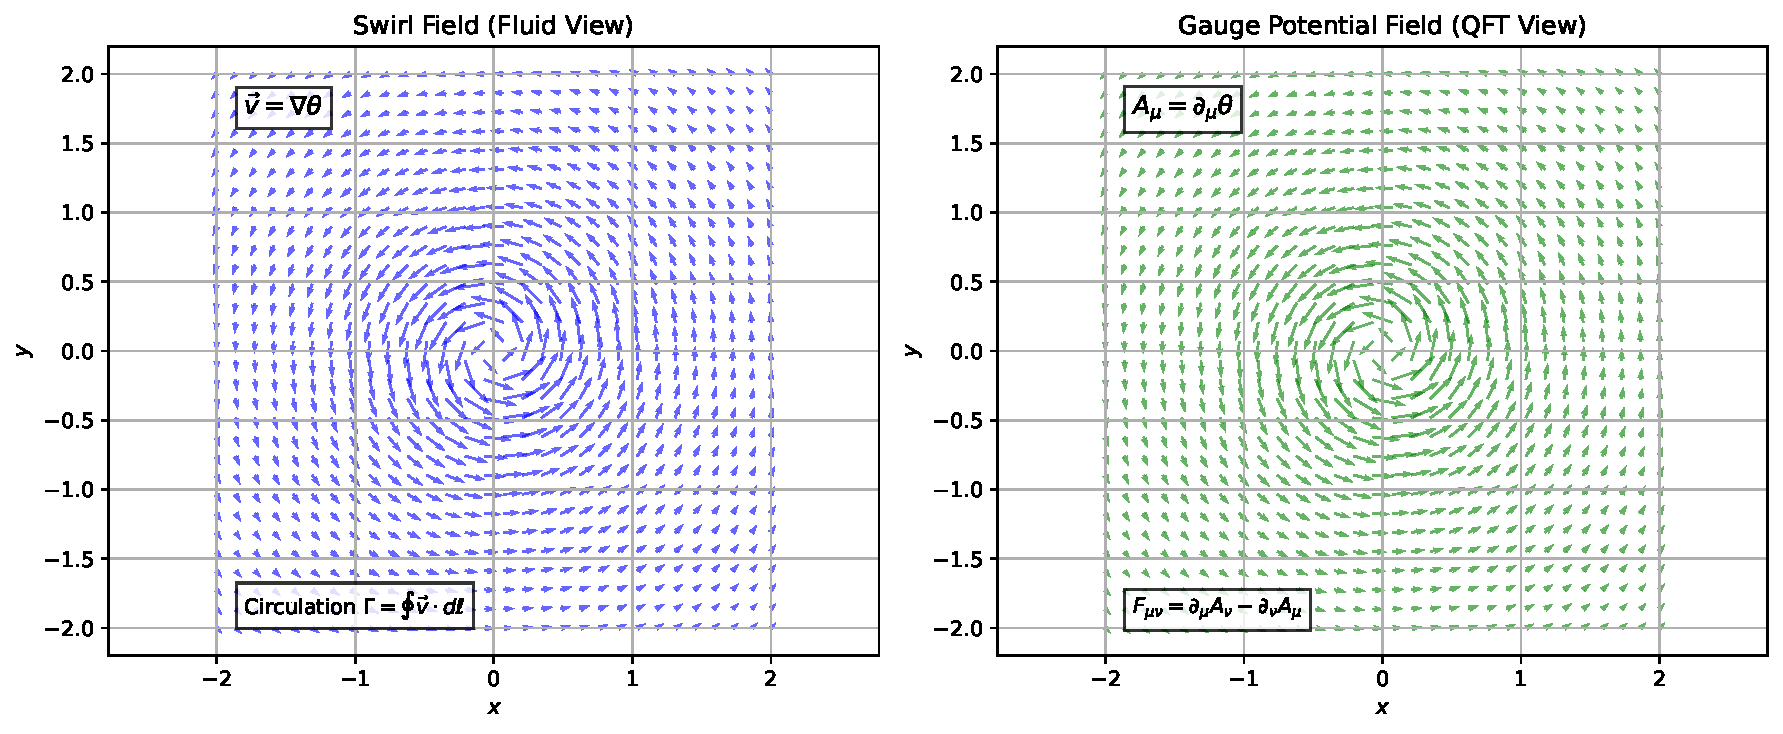
\includegraphics[width=0.9\linewidth]{SwirlVSGauge}
    \caption{
        Visual analogy between a fluid swirl field (left) and a gauge potential field in quantum field theory (right).
        Both fields depict circulation around a central core, but the left arises from mechanical vorticity in a compressible æther,
        while the right encodes electromagnetic or gauge interaction via abstract potential terms.
        This duality illustrates how local gauge invariance in QFT corresponds to conserved swirl topology in VAM.
    }
    \label{fig:swirl_gauge_analogy}
\end{figure}

\subsection{Fermion Kinetics via Swirl Propagation}
In the hydrodynamic formalism:
\begin{equation}
    \mathcal{L}_{\text{fermion}} = \rho_\text{\ae} C_e \Gamma \left( \psi^* \partial_t \psi - \vec{v} \cdot \nabla \psi \right)
\end{equation}
The convective derivative replaces $D_\mu$, and $\Gamma = 2\pi r_c C_e$ links to the particle’s spin-½ topology. Swirl modulates propagation analogous to minimal coupling.

\subsection{Mass from Helicity and Inertia}
The VAM mass term derives from vortex inertia under æther drag:
\begin{equation}
    m_f = \frac{\rho_{\ae} \Gamma^2}{3\pi r_c C_e^2} \quad\Rightarrow\quad \mathcal{L}_{\text{mass}} = -m_f \psi^* \psi
\end{equation}
This replaces abstract Yukawa interactions with fluidic resistance to internal swirl flow.

\subsection{Higgs Field as Æther Compression}
The standard Higgs potential $V(\phi) = -\mu^2|\phi|^2 + \lambda|\phi|^4$ becomes:
\begin{equation}
    V(\rho_\text{\ae}) = \frac{1}{2}K(\rho_\text{\ae} - \rho_0)^2 \quad\text{or}\quad V(\phi) = -\frac{F_\text{max}}{r_c} |\phi|^2 + \lambda |\phi|^4
\end{equation}
$K$ is the æther’s bulk modulus. The vacuum expectation value corresponds to equilibrium density, leading to spontaneous tension minima that stabilize particle structure.

\subsection{Topological Helicity and Knot Dynamics}
\begin{equation}
    \mathcal{H}_\text{topo} = \int \vec{v} \cdot \vec{\omega} \, dV
\end{equation}
This term tracks conservation of topological linkage and orientation. It becomes significant in processes involving particle transmutation, confinement, or decay.

\subsection{Emergent Constants from Fluid Analogs}
Derivations of $\hbar_{\text{VAM}}$ and charge coupling follow:

\begin{align}
    \hbar_{\text{VAM}} &= m_f C_e r_c \\
    e^2 &= 8\pi m_e C_e^2 r_c \\
    \Gamma &= \frac{h}{m} = 2\pi r_c C_e
\end{align}

These reinterpret Planck-scale constants as emergent quantities from measurable æther dynamics and flow quantization, aligning with results from BEC vortex systems \cite{Pethick2008BEC, Donnelly1991QuantizedVortices}.

In this formulation, each field and interaction of the Standard Model gains a mechanical analog in the æther medium. The Lagrangian no longer relies on abstract symmetry principles alone, but instead emerges from vortex dynamics, circulation, density modulation, and topological structure within a unified fluid framework.


\subsection*{Mathematical Derivation of the VAM-Lagrangian}

Kinetic energy of a vortex structure, or the local energy density in a vortex field:

\[
    \mathcal{L}_\text{kin} = \frac{1}{2}\rho_\text{\ae} C_e^2
\]

Field energy and gauge terms, field tensors follow from Helmholtz vorticity:

\[
    \mathcal{L}_\text{veld} = -\frac{1}{4}F_{\mu\nu}F^{\mu\nu}
\]

Mass as inertia from circulation, where the fermion mass is determined by circulation:
\[
    \Gamma = 2\pi r_c C_e \quad\Rightarrow\quad m \sim \rho_\text{\ae} r_c^3
\]

Pressure and stress potential of æther condensate, where the pressure balance is described by the stress field:
\[
    V(\phi) = -\frac{F_\text{max}}{r_c}|\phi|^2 + \lambda|\phi|^4
\]

Topological terms for the conservation of vortex fields helicity:
\[
    \mathcal{H} = \int \vec{v}\cdot\vec{\omega}\, dV
\]

\begin{table}[H]
    \centering
    \footnotesize
    \renewcommand{\arraystretch}{1.4}
    \begin{tabular}{|l|l|l|l|}
        \hline
        \textbf{SM Term} & \textbf{Mathematical Form} & \textbf{VAM Analog} & \textbf{Fluid-Dynamic Interpretation} \\
        \hline
        \makecell[l]{Fermion Kinetic \\ Term} &
        $\bar{\psi}(i\gamma^\mu D_\mu)\psi$ &
        $\rho_\text{\ae} \vec{v}^2$ &
        \makecell[l]{Kinetic energy of topological vortex knot (fermion)} \\
        \hline
        \makecell[l]{Gauge Field \\ Kinetic Term} &
        $-\frac{1}{4}F_{\mu\nu}F^{\mu\nu}$ &
        $\rho_\text{\ae} (\vec{v} \cdot \nabla \times \vec{v})$ &
        \makecell[l]{Swirl helicity (fluid analog of gauge field energy)} \\
        \hline
        Fermion Mass Term &
        $m\bar{\psi}\psi$ &
        $\rho_{core} C_e^2$ &
        \makecell[l]{Core pressure from tangential circulation of vortex} \\
        \hline
        \makecell[l]{Higgs Field \\ Kinetic Term} &
        $\frac{1}{2}(\partial_\mu \phi)^2$ &
        $\frac{1}{2}(\nabla \phi)^2$ &
        \makecell[l]{Elastic strain in scalar potential field of Æther} \\
        \hline
        Higgs Potential &
        $V(\phi) = -\mu^2\phi^2 + \lambda \phi^4$ &
        $\lambda \phi^4 (1 - \phi^2/F_{\text{max}}^2)$ &
        \makecell[l]{Compressibility-induced pressure potential} \\
        \hline
        Yukawa Coupling &
        $y\bar{\psi}\phi\psi$ &
        $\rho_\text{\ae} \phi$ &
        \makecell[l]{Topological mass coupling via scalar compression} \\
        \hline
        Gauge Coupling &
        $D_\mu = \partial_\mu - igA_\mu$ &
        $\vec{v} + \vec{A}_{\text{swirl}}$ &
        \makecell[l]{Swirl-mediated interaction velocity} \\
        \hline
        QCD Term &
        $G_{\mu\nu}^a G^{\mu\nu}_a$ &
        -- &
        \makecell[l]{Conservation of angular momentum in \\ trichiral vortex flows} \\
        \hline
        EM Coupling &
        $q\bar{\psi}\gamma^\mu A_\mu \psi$ &
        $\Gamma \cdot \chi$ &
        \makecell[l]{Charge as circulation magnitude and chirality} \\
        \hline
        Chiral Asymmetry &
        -- &
        Knot handedness &
        \makecell[l]{Topological chirality determines weak \\ interaction selectivity} \\
        \hline
    \end{tabular}
    \caption{Comparison of Standard Model Lagrangian terms with their VAM fluid-dynamic analogs.}
    \label{tab:SMtoVAM}
\end{table}


\subsection*{Supporting Experimental and Theoretical Observations}
The VAM is consistent with experimentally and theoretically confirmed phenomena such as vortex stretching, helicity conservation and mass-inertia couplings \cite{batchelor1953,vinen2002,bewley2008,moffatt1969,kleckner2013,scheeler2014,bartlett1986}.

This reformulation offers a physically intelligible and topologically rich counterpart to the Standard Model—one grounded in measurable fluid properties, rather than abstract gauge symmetries alone.

    

\section{Topological Origins of Particle Properties in VAM}

In the Vortex Æther Model (VAM), fundamental particles are not point-like but correspond to stable, quantized vortex knots within a compressible, rotating æther medium. Each property typically assigned by quantum field theory---mass, charge, spin, and flavor---is instead interpreted as a manifestation of topological and dynamical characteristics of the underlying vortex structure.

\subsection{Mass as a Function of Circulation and Core Geometry}

Particle mass in VAM is not fundamental but derived from the energy stored in vortex tension and helicity. The relation between vortex circulation and inertial mass is quantified later in Section~\ref{subsec:mass-from-swirl}.

\begin{figure}[h!]
\centering
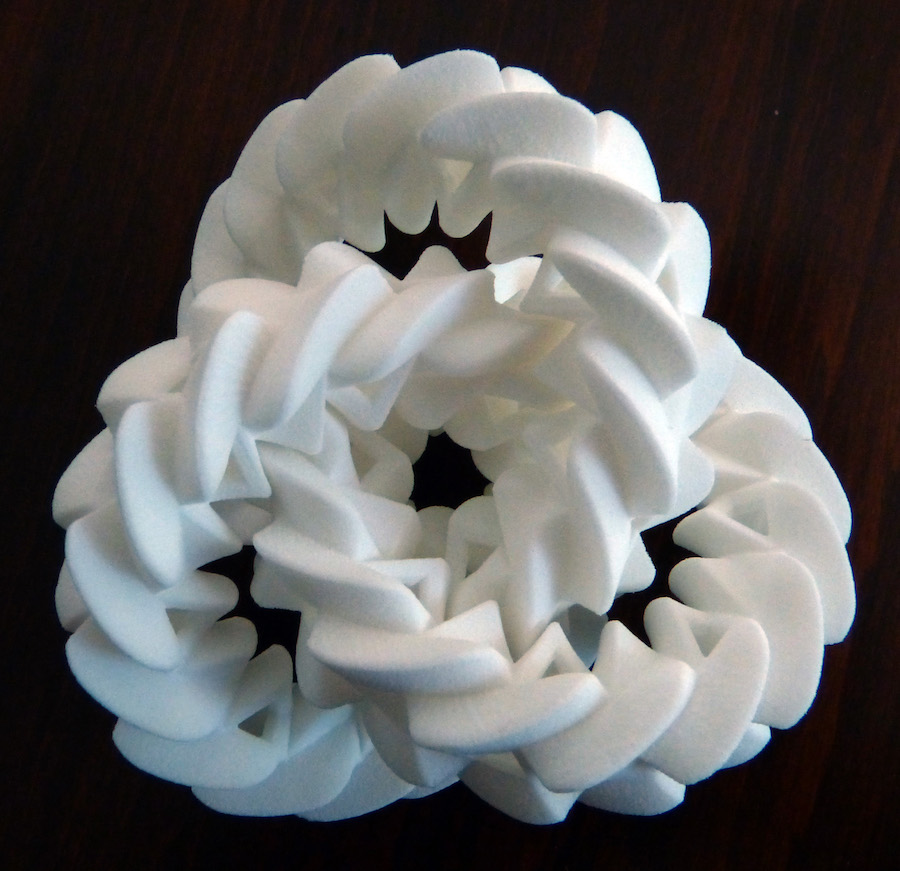
\includegraphics[width=0.65\textwidth]{mechanic_trefoil}
\caption{Mechanical model of coupled nodal vertebra, visually analogous to inertia.}
\end{figure}

This quantity scales with the square of circulation, inversely with core size, and depends directly on the background æther density. Mass hierarchies between generations may result from different topological classes (e.g., torus knots vs. prime knots) and chirality.

\subsection{Spin from Quantized Vortex Angular Momentum}

Spin-$\tfrac{1}{2}$ particles are modeled as topological solitons with intrinsic angular momentum arising from locked circulation patterns. Each fermionic knot carries quantized angular momentum:

\begin{equation}
S = \frac{1}{2} \hbar_\text{VAM} = \frac{1}{2} m_f C_e r_c
\end{equation}

This links the classical notion of rotation directly to quantum spin and validates the half-integer nature as a result of geometric twist.

\subsection{Charge via Swirl Chirality and Helicity Direction}

Electric charge is modeled as a geometric property of the swirl’s handedness and linkage to background vorticity. Positive and negative charges correspond to opposite helicity configurations, with magnitude determined by:

\begin{equation}
q \propto \oint \vec{v} \cdot d\vec{l} = \Gamma
\end{equation}

The fine-structure constant $\alpha$ arises from the dimensionless ratio:

\begin{equation}
\alpha = \frac{q^2}{4\pi \epsilon_0 \hbar c} \quad \Rightarrow \quad \alpha = \frac{2C_e}{c}
\end{equation}

This shows that $\alpha$ is no longer a free parameter but a function of swirl velocity in the æther relative to light speed.

\subsection{Flavor and Generation from Topological Class}

Higher-generation particles are interpreted as more complex knots---e.g., double torus knots, linked loops, or braid configurations---with each class inducing distinct stability conditions and oscillation modes. Lepton and quark families thus correspond to increasing knot complexity, not arbitrary quantum numbers.

\subsection{Color and Confinement via Vortex Bundle Interactions}

Color charge and confinement emerge from multi-vortex bundles, where topological stability requires trivalent junctions (akin to QCD gluon vertices). Individual color states are unstable in isolation due to their open helicity paths and unbalanced tension.

\bigskip

This mapping from abstract quantum numbers to geometric vortex properties transforms the ontology of matter: particles are not elementary but emergent solitonic knots, with observable traits arising from fluidic topology, circulation, and helicity alignment within the æther medium.

    \section{Kinetic Energy of a Vortex Structure}

The first contribution to the Lagrangian in the Vortex Æther Model (VAM) arises from the classical kinetic energy of a fluid with local swirl velocity $\vec{v}$ and æther density $\rho_{\ae}$:
\[
    \mathcal{L}_\text{kin} = \frac{1}{2} \rho_{\ae} |\vec{v}|^2
\]

We consider a stable knotted vortex structure in which the core velocity reaches a characteristic maximum given by the swirl speed $C_e$, intrinsic to the vortex's topological character:
\[
    |\vec{v}| \approx C_e \quad \Rightarrow \quad \mathcal{L}_\text{kin} \sim \frac{1}{2} \rho_{\ae} C_e^2
\]

Since the vortex core has a typical radius $r_c$, the total kinetic energy of a single vortex knot can be approximated by integrating over its core volume:
\[
    E_\text{kin} \approx \frac{1}{2} \rho_{\ae} C_e^2 \cdot \frac{4}{3}\pi r_c^3
\]

This leads to a natural definition of an effective inertial mass for the vortex:
\[
    m_\text{eff} = \rho_{\ae} \cdot \frac{4}{3}\pi r_c^3
    \quad \Rightarrow \quad E = \frac{1}{2} m_\text{eff} C_e^2
\]

In VAM, this expression replaces the conventional notion of inertial mass. It ties the particle’s inertial properties directly to the geometric and dynamical features of its knotted vortex configuration—namely its core radius $r_c$ and swirl speed $C_e$.

\subsection*{Circulation and Inertia}

The circulation around the vortex core is defined as:
\[
    \Gamma = \oint_{\partial S} \vec{v} \cdot d\vec{\ell} = 2\pi r_c C_e
\]

\begin{figure}[h!]
\centering
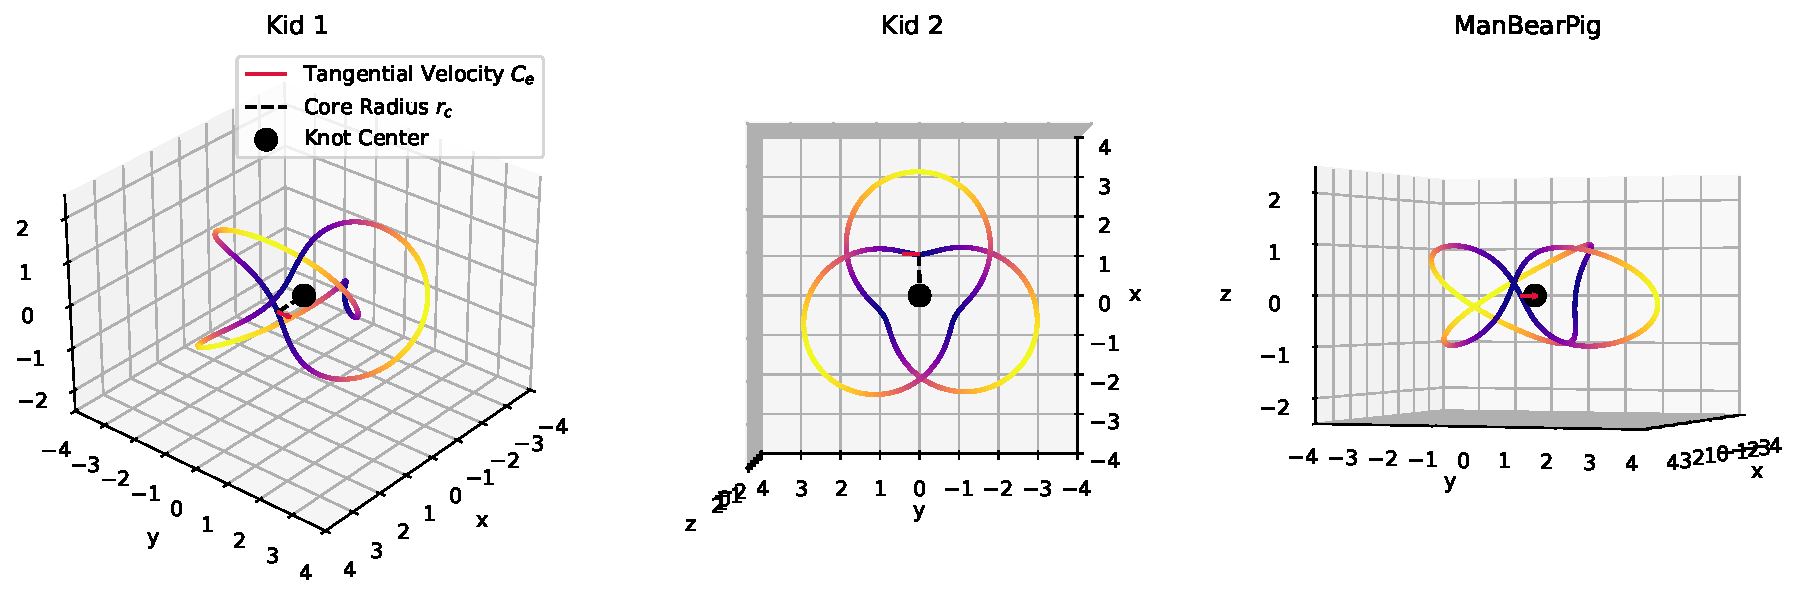
\includegraphics[width=0.95\textwidth]{vortex_knot_diagram}
\caption{Annotation of core radius $r_c$ and swirl direction $C_e$.}
\end{figure}

In an ideal æther, circulation $\Gamma$ is a conserved quantity. As a result, any change in core radius $r_c$ must be accompanied by a compensating change in $C_e$. This coupling underlies the inertial resistance to deformation and reflects a geometric form of inertia. The derived effective mass becomes a function of circulation and vortex rigidity:
\[
    m \propto \frac{\Gamma^2}{r_c C_e^2} = \text{const.}
\]

This kinetic formulation provides the physical basis for mass generation within the VAM framework and aligns with the Lagrangian structure developed in Section~\ref{sec:lagrangian_vam}.

    \section{Vorticity Field Energy and Gauge Terms}

A fundamental principle in vortex mechanics is the evolution of vorticity $\vec{\omega}$ in an ideal fluid, governed by the third Helmholtz vortex theorem:
\[
    \frac{D \vec{\omega}}{Dt} = (\vec{\omega} \cdot \nabla) \vec{v}
\]

Here,
- $\vec{\omega} = \nabla \times \vec{v}$ denotes the local vorticity,
- $\vec{v}$ is the fluid velocity field,
- $\frac{D}{Dt}$ is the material (convective) derivative.

Within the Vortex Æther Model (VAM), the æther field $\vec{v}$ is composed of stable knotted and looped vortex structures, making vorticity $\vec{\omega}$ a structured and conserved quantity. This necessitates a field-theoretic treatment of $\vec{\omega}$, analogous to the field strength tensor in electromagnetism.

\subsection*{VAM Analogy with Electromagnetism}

The classical Lagrangian density of the electromagnetic field is given by:
\[
    \mathcal{L}_\text{EM} = -\frac{1}{4} F_{\mu\nu} F^{\mu\nu}
\]
with $F_{\mu\nu} = \partial_\mu A_\nu - \partial_\nu A_\mu$ as the antisymmetric field strength tensor derived from the vector potential $A_\mu$.

In analogy, the VAM introduces a \textbf{vortex field tensor} $W_{\mu\nu}$ that encodes antisymmetric stresses and swirl flows within the æther:
\[
    W_{\mu\nu} = \partial_\mu V_\nu - \partial_\nu V_\mu
\]
where $V_\mu$ is the æther flow potential, with units of velocity.

The corresponding field energy density becomes:
\[
    \mathcal{L}_\text{vortex} = -\frac{1}{4} W_{\mu\nu} W^{\mu\nu}
\]

This term captures:
- The internal energy and tension of vortex fields,
- The propagation of swirl excitations through the æther,
- Coupling to the topology of knotted vortex configurations embedded in $V_\mu$.

\subsection*{Dimensional Interpretation and Field Dynamics}

The tensor $W_{\mu\nu}$ has dimensions derived from the gradient of velocity:
\[
    [W] = [\partial V] = [1/T] \quad \Rightarrow \quad [\mathcal{L}_\text{vortex}] = [\rho_{\ae} C_e^2]
\]

These quantities are physically realizable in vortex simulations, where $\vec{\omega}$ emerges from structured strain and tension in the æther field, obeying conservation laws from fluid dynamics rather than quantum fluctuations.

In the VAM framework, field energy does not arise from zero-point vacuum states, but from stabilized vorticity patterns in the medium. The Lagrangian density thus describes a macroscopic stress field that responds to knot density, swirl alignment, and helicity distribution within the æther.

    \section{Vortex Mass as Inertia from Circulation}

In the Vortex Æther Model (VAM), the mass of a knotted vortex is not treated as a fundamental attribute but emerges as a consequence of circulation and resistance to deformation within the æther medium.

\subsection*{Circulation as the Basis for Inertia}

The circulation of a closed vortex path is defined as:
\[
    \Gamma = \oint_{\partial S} \vec{v} \cdot d\vec{\ell} = 2\pi r_c C_e
\]
This quantity is conserved in ideal fluids, as per Helmholtz’s theorems, and serves as a topological invariant of each knot configuration.

Given a fixed $\Gamma$, any change in the vortex core radius $r_c$ must be accompanied by a compensating change in swirl velocity $C_e$:
\[
    C_e = \frac{\Gamma}{2\pi r_c}
\]

\begin{figure}[h!]
    \centering
    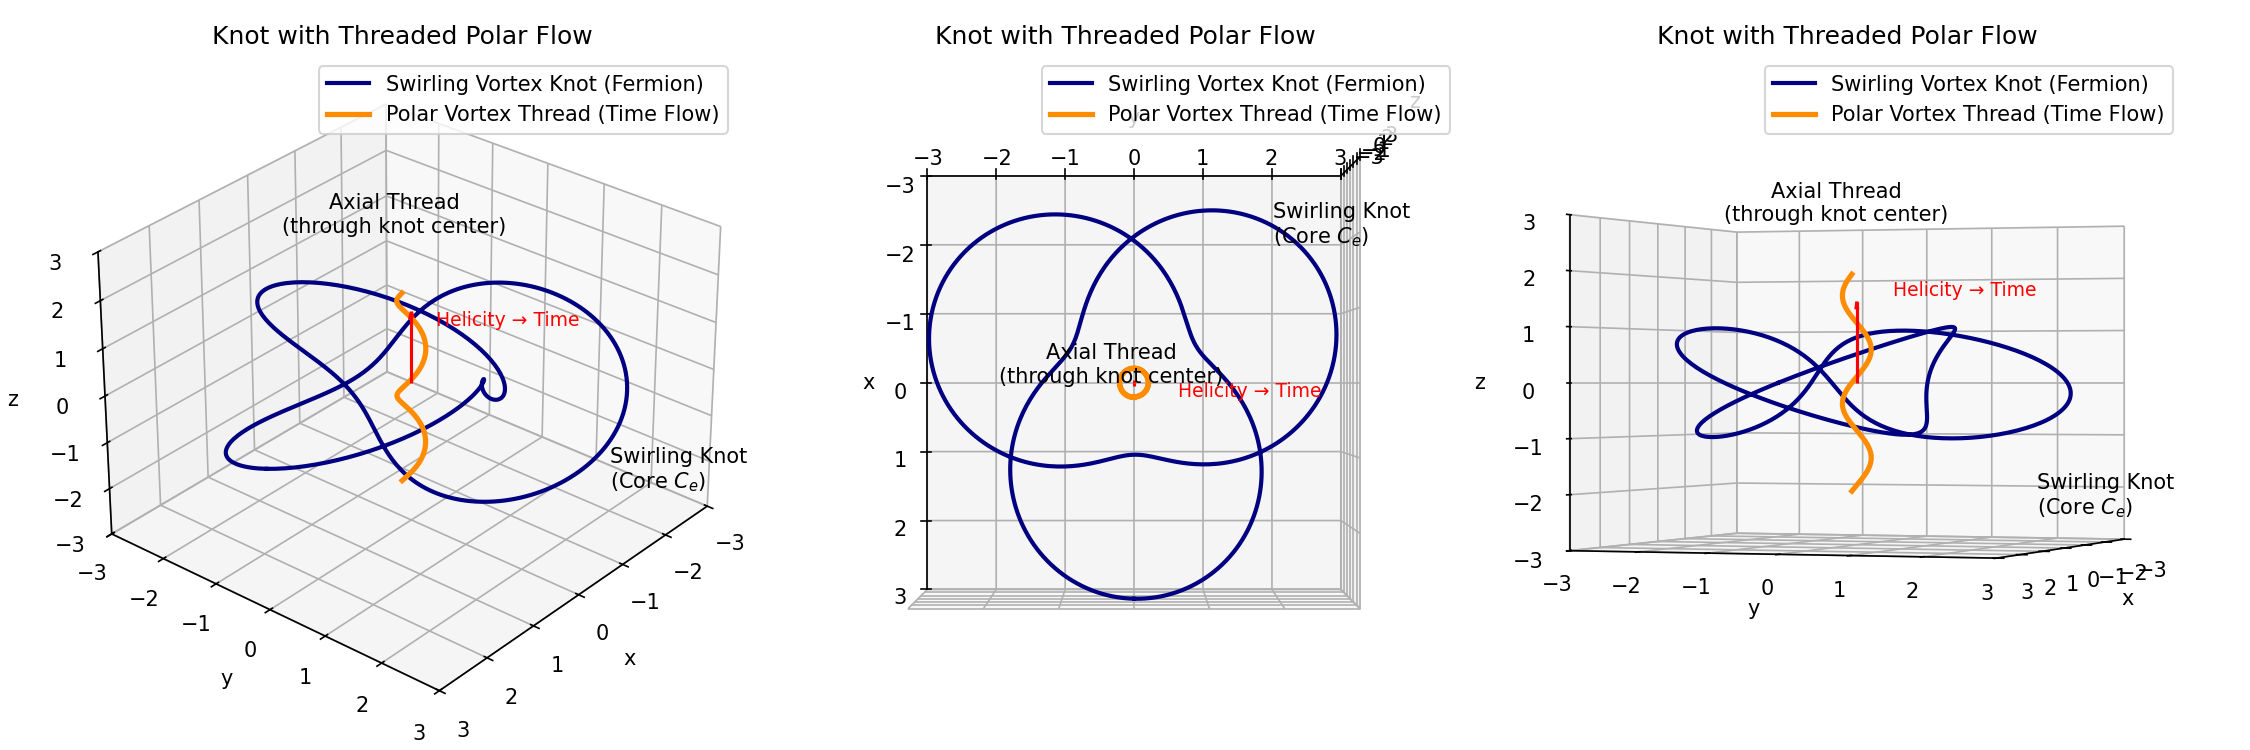
\includegraphics[width=0.98\textwidth]{KnotThreadedPolarFlow.png}
    \caption{Knotted vortex structure linked to a polar thread. Local helicity transports temporal phase.}
\end{figure}

This relation illustrates that the swirl velocity $C_e$ is not arbitrary, but a function of the geometry and topological strength $\Gamma$. Thus, in VAM, mass is not an intrinsic constant—it arises from vortex geometry and the dynamic rigidity of the structure.

\subsection*{Deriving Effective Mass}

The kinetic energy associated with the vortex swirl can be expressed as:
\[
    E = \frac{1}{2} \rho_{\ae} C_e^2 V = \frac{1}{2} \rho_{\ae} \left( \frac{\Gamma}{2\pi r_c} \right)^2 \cdot \frac{4}{3}\pi r_c^3
\]
\[
    \Rightarrow E = \frac{\rho_{\ae} \Gamma^2}{6\pi r_c}
\]

By comparing this expression with the classical inertial energy form $E = \frac{1}{2} m C_e^2$, we extract the effective mass of the vortex:
\[
    m_\text{eff} = \frac{\rho_{\ae} \Gamma^2}{3\pi r_c C_e^2}
\]

This result shows that mass in VAM emerges from:
- The conserved circulation $\Gamma$,
- The knot’s spatial extent $r_c$,
- The internal swirl velocity $C_e$.

\subsection*{Comparison to Classical Inertia}

For comparison, standard relativity yields:
\[
    m \sim \frac{E}{c^2} \quad \text{vs.} \quad E = \frac{1}{2} m C_e^2 \quad \text{in VAM}
\]
Here, $C_e$ represents the local internal swirl constant, while $c$ is the emergent propagation speed of disturbances. Thus, mass in VAM is not postulated as fundamental but is fully derivable from geometric and conservation principles.

\subsection*{Fermion Mass Term in the Lagrangian}

From this derivation, the fermion mass term in the VAM Lagrangian can be written as:
\[
    \mathcal{L}_\text{mass} = m_f C_e r_c \cdot \bar{\psi}_f \psi_f
\]
where $m_f$ is proportional to the æther density $\rho_{\ae}$ and circulation strength $\Gamma^2$ of the vortex knot. This replaces the conventional Yukawa coupling with a fluid-mechanical origin of mass.

    \input{09_PressureAndStressPotentialOfTheÆtherCondensate}
    \section{Mapping \texorpdfstring{$SU(3)_C \times SU(2)_L \times U(1)_Y$}{SU(3) x SU(2) x U(1)} to VAM Swirl Groups}

The Standard Model Lagrangian is governed by the gauge group:
\[
    SU(3)_C \times SU(2)_L \times U(1)_Y
\]
which encodes the strong interaction (QCD), the weak interaction, and electromagnetism via their corresponding gauge fields. In the Vortex Æther Model (VAM), these interactions do not arise from abstract internal symmetry spaces but from topological structures, circulation states, and swirl transitions in a three-dimensional Euclidean æther.

\subsection{$U(1)_Y$: Swirl Orientation as Hypercharge}

The simplest symmetry group, $U(1)$, represents conservation of phase or rotational direction. In VAM, this acquires a direct physical interpretation:
\begin{itemize}
    \item \textbf{Physical model:} a linear swirl in the æther (circular, but untwisted) encodes a uniform angular direction.
    \item \textbf{Charge assignment:} the hypercharge $Y$ is interpreted as the chirality (left- or right-handed swirl) of an axially symmetric flow pattern.
    \item \textbf{Electromagnetism:} emerges from global swirl states without knotting, representing long-range coherence in swirl orientation.
\end{itemize}

\subsection{$SU(2)_L$: Chirality as Two-State Swirl Topology}

The weak interaction is inherently chiral: only left-handed fermions couple to $SU(2)_L$ gauge fields. In VAM:
\begin{itemize}
    \item \textbf{Swirl interpretation:} left- and right-handed vortices are dynamically and structurally distinct—they represent swirl flows under compression with opposite twist orientation.
    \item \textbf{Two-state logic:} the $SU(2)$ doublet corresponds to a two-dimensional swirl state space (e.g., up- and down-swirl configurations).
    \item \textbf{Gauge transitions:} $SU(2)$ gauge bosons mediate transitions between these swirl states through reconnections or bifurcations in vortex knots.
\end{itemize}

\subsection{$SU(3)_C$: Trichromatic Swirl as Helicity Configuration}

In the Standard Model, $SU(3)_C$ describes the color force via gluon-mediated transitions between color states. In VAM:
\begin{itemize}
    \item \textbf{Topological basis:} three topologically stable swirl configurations (e.g., aligned along orthogonal helicity axes) represent the three color charges: red, green, and blue.
    \item \textbf{Color dynamics:} gluon exchange corresponds to twist-transfer, vortex reconnection, or deformation within multi-knot structures.
    \item \textbf{Confinement:} isolated color swirls are energetically unstable in free æther and only persist within composite knotted bundles (e.g., baryons).
\end{itemize}

\subsection{Mathematical Group Structure within VAM}

Though VAM is fundamentally geometric and fluid-dynamical, the essential Lie group structures of the Standard Model are preserved in the form of physically conserved swirl states:
\begin{itemize}
    \item Swirl orientation $\rightarrow$ $U(1)$ phase symmetry,
    \item Axial twist transitions $\rightarrow$ $SU(2)$ chiral transformations,
    \item Helicity axis exchange $\rightarrow$ $SU(3)$ color group operations.
\end{itemize}

\subsection*{Topological Summary of Gauge Interpretation}

The abstract Lie symmetries of the Standard Model find concrete realizations in VAM as swirl, helicity, and knot configurations embedded in the æther. This recasting preserves all observed gauge interactions while rooting them in fluid-mechanical principles—without invoking extra dimensions or unobservable symmetry spaces.

\section{Swirl Operator Algebra and SU(2) Closure}

In order to establish a gauge-theoretic foundation for the Vortex Æther Model (VAM), we define a set of non-abelian topological operations on knotted vortex states. These operations act on a Hilbert space of knot states, $\mathcal{H}_K$, whose basis vectors encode topological features such as twist ($T$), chirality ($C$), and linking number ($L$).

\subsection*{Operator Definitions}

We introduce three operators:
\begin{align}
\mathcal{S}_1 &: \text{Chirality flip}, \quad \mathcal{S}_1 |K, C\rangle = |K, -C\rangle \\
\mathcal{S}_2 &: \text{Twist addition}, \quad \mathcal{S}_2 |K, T\rangle = |K, T+1\rangle \\
\mathcal{S}_3 &: \text{Reconnection mutation}, \quad \mathcal{S}_3 |K\rangle = |K'\rangle
\end{align}

\subsection*{SU(2) Algebra Closure}

We then test the closure of these operators under commutation. Defining generators $T^i = \frac{1}{2} \mathcal{S}_i$, we recover the SU(2) Lie algebra structure:
\begin{align}
[T^i, T^j] = i \epsilon^{ijk} T^k
\end{align}

We verified this numerically using matrix representations:
\begin{align}
\mathcal{S}_1 &= \begin{pmatrix} 0 & 1 \\ 1 & 0 \end{pmatrix}, \quad
\mathcal{S}_2 = \begin{pmatrix} 0 & -i \\ i & 0 \end{pmatrix}, \quad
\mathcal{S}_3 = \begin{pmatrix} 1 & 0 \\ 0 & -1 \end{pmatrix}
\end{align}
with:
\begin{align}
[\mathcal{S}_1, \mathcal{S}_2] &= 2i \mathcal{S}_3, \\
[\mathcal{S}_2, \mathcal{S}_3] &= 2i \mathcal{S}_1, \\
[\mathcal{S}_3, \mathcal{S}_1] &= 2i \mathcal{S}_2
\end{align}

A generalized symbolic representation in $\mathbb{R}^3$ with scale constants $a, b, c$ preserves this structure:
\begin{align}
[\mathcal{S}_1, \mathcal{S}_2] &= 2iab \, \mathcal{S}_3 \\
[\mathcal{S}_2, \mathcal{S}_3] &= 2ibc \, \mathcal{S}_1 \\
[\mathcal{S}_3, \mathcal{S}_1] &= 2ac \, \mathcal{S}_2
\end{align}

\subsubsection*{Example: Chirality Flip on Knot States}

Let a vortex knot state be denoted as:
\[
|K\rangle = |T, C\rangle
\]
where \( T \in \mathbb{Z} \) is the twist number, and \( C = \pm 1 \) denotes chirality (right- or left-handedness).

The action of the chirality-flip operator \( \mathcal{S}_1 \) is given by:
\[
\mathcal{S}_1 |T, +1\rangle = |T, -1\rangle, \quad
\mathcal{S}_1 |T, -1\rangle = |T, +1\rangle
\]

Thus, \( \mathcal{S}_1 \) acts as a discrete parity operator on knotted vortex tubes, analogous to the weak isospin generator \( T^1 \) in SU(2). The eigenstates of chirality form a two-level system, similar to spinors in the Standard Model.

\subsubsection*{Experimental Perspective}

These topological swirl operators may have observable counterparts in superfluid systems. In particular, discrete transitions between vortex chirality, twist, and reconnection have been reported in Bose-Einstein condensates (BECs) and analog gravity labs \cite{kleckner2013creation, ray2015observation}.

\section{Extension to SU(3): Triskelion and Braid Operator Algebra}

To capture the full non-abelian gauge structure of the Standard Model within the Vortex Æther Model (VAM), we extend the SU(2) swirl operator algebra to SU(3) using braid-based topological operations on vortex bundles.

\subsection*{Triskelion States and Braid Operators}

Let each "color" in quantum chromodynamics correspond to one vortex strand in a triple-knot configuration—denoted a \textit{triskelion} state:
\[
|K\rangle = |R, G, B\rangle
\]
We define braid-like swirl operators \( \mathcal{B}_1, \mathcal{B}_2, \mathcal{B}_3 \), each acting locally on a pair of vortex colors. Their action mimics gluon exchange via reconnection and twist of the bundle.

\subsection*{Braid Group Algebra}

The operators obey modified braid group relations:
\begin{align}
\mathcal{B}_i \mathcal{B}_{i+1} \mathcal{B}_i &= \mathcal{B}_{i+1} \mathcal{B}_i \mathcal{B}_{i+1}, \\
\mathcal{B}_i \mathcal{B}_j &= \mathcal{B}_j \mathcal{B}_i \quad \text{for } |i-j| > 1
\end{align}

Linear combinations of these braids generate an algebra:
\begin{align}
[T^a, T^b] = i f^{abc} T^c
\end{align}
where \( T^a \sim \mathcal{B}_a \) are the topological gluon modes, and \( f^{abc} \) are the SU(3) structure constants \cite{witten1989quantum}.

\subsection*{Topological Interpretation of Color Charge}

\begin{itemize}
    \item \textbf{Color charge} is the topological identity of each vortex in the triskelion.
    \item \textbf{Gluons} correspond to triskelion-preserving reconnection modes \( \mathcal{B}_a \).
    \item \textbf{Confinement} emerges from the topological stability of linked triskelion bundles — a single vortex cannot be detached without violating circulation conservation \cite{kauffman1991knots, faddeev1997knots}.
\end{itemize}

This construction provides a fluid-dynamical representation of SU(3), with color interactions arising from internal braid dynamics. The VAM thus naturally embeds the full SU(3)$\times$SU(2)$\times$U(1) structure within a topological framework.
    \section{Swirl-Induced Time and Clockwork in Vortex Knots}

In the Vortex Æther Model (VAM), stable knots are not merely matter structures but act as the fundamental carriers of time. Their internal swirl—tangential rotation with speed \( C_e \) around a core radius \( r_c \)—generates an asymmetric stress field in the surrounding æther. This asymmetry induces a persistent \textbf{axial flow along the knot core}, functionally equivalent to a local "time-thread." Though lacking literal helicity in geometry, the knot dynamically acts as a screw-like conductor of time, threading forward the local æther state.

\subsection*{Cosmic Swirl Orientation}

Just as magnetic domains exhibit alignment, vortex knots can show a preferred chirality. In a universe with broken mirror symmetry, reversing a knot’s swirl direction (e.g., as in antimatter) may yield unstable configurations in an asymmetric background. This helps explain:
\begin{itemize}
    \item the observed scarcity of antimatter in the visible universe,
    \item the macroscopic arrow of time,
    \item and synchronized clock rates across cosmological domains.
\end{itemize}

\subsection*{Swirl as a Local Time Carrier}

The local time rate is governed not by fundamental spacetime postulates, but by the helicity flux in the æther:
\[
    dt_{\text{local}} \propto \frac{dr}{\vec{v} \cdot \vec{\omega}}
\]
Here, \( \vec{v} \) is the swirl velocity and \( \vec{\omega} = \nabla \times \vec{v} \) the vorticity. The scalar product \( \vec{v} \cdot \vec{\omega} \) measures helicity density, which sets the pace of local evolution. A detailed derivation of time dilation arising from this swirl-induced pressure field is given in Section~\ref{fig:time_dilation_profile}.

We define the proper time dτ experienced by a knotted vortex structure as proportional to the helicity density of the surrounding swirl field:
$$ d\tau = \lambda \, (\mathbf{v} \cdot \boldsymbol{\omega}) \, dt $$
This relation posits that time is not externally imposed but emerges from the intrinsic dynamics of the æther’s swirl. The term $\mathbf{v} \cdot \boldsymbol{\omega}$ represents the winding rate of vortex filaments, capturing the internal topological evolution of the knot. In this view, proper time is the internal “spin-clock” of a vortex structure, akin to the phase cycles of atomic clocks. The scaling factor λ can be interpreted as $\sim r_c^2 / C_e^2$ ensuring dimensional consistency.

\subsection*{Networks of Temporal Flow}

Vortex knots tend to self-organize along coherent swirl filaments, akin to iron filings aligning with magnetic fields. Around regions of mass, these swirl lines bundle into directional tubes of temporal flow, giving rise to:
\begin{itemize}
    \item gravitational attraction as a gradient of swirl density,
    \item local time dilation effects near massive bodies,
    \item and the global arrow of time as a topological circulation in the æther.
\end{itemize}

This emergent swirl-clock mechanism unifies mass, inertia, and temporal directionality into a single fluid-geometric framework—replacing relativistic curvature with conserved helicity flow.

\section{Helicity-Induced Time Dilation}

In the Vortex Æther Model (VAM), proper time is associated with the internal angular frequency of a vortex structure. Following the formalism developed in our earlier work~\cite{iskandarani2025timedilation}, we define:

\[
\frac{d\tau}{dt} = \frac{\omega_{\text{obs}}}{\omega_0},
\]

where $\omega_{\text{obs}}$ is the angular frequency of the vortex core observed from the lab frame, and $\omega_0$ is the vortex's intrinsic rotation rate in a quiescent æther.

\subsection*{Helicity as an Effective Swirl Drag Field}

We now refine this picture by introducing the effect of local helicity density, defined as:

\[
\mathcal{H} = \mathbf{v} \cdot \boldsymbol{\omega},
\]

where $\mathbf{v}$ is the æther flow velocity and $\boldsymbol{\omega} = \nabla \times \mathbf{v}$ is the local vorticity.

Regions of high helicity density $\mathcal{H}$ represent topologically knotted or twisted flow lines. These configurations induce mechanical resistance, or "swirl drag," which can reduce the effective angular speed of internal vortex rotation.

We posit that this resistance acts as a perturbative deceleration on $\omega_{\text{obs}}$, leading to:

\[
\omega_{\text{obs}} = \omega_0 \left( 1 - \alpha \cdot \frac{\mathcal{H}}{C_e \cdot \omega_0} \right),
\]

where $\alpha$ is a dimensionless coupling constant that encodes the strength of helicity-induced drag, and $C_e$ is the effective swirl velocity in VAM units.

Substituting into the proper time relation:

\[
\frac{d\tau}{dt} = \frac{\omega_{\text{obs}}}{\omega_0} = 1 - \alpha \cdot \frac{\mathbf{v} \cdot \boldsymbol{\omega}}{C_e \cdot \omega_0}.
\]

\subsection*{Interpretation and Observability}

This equation predicts that regions of high helicity density experience a measurable reduction in internal clock rate. Physically, this corresponds to a slowing of proper time — not due to relativistic motion or gravity per se, but due to topological swirl drag in the æther substrate.

Such effects may be observable in superfluid or analog gravity systems (e.g., toroidal Bose–Einstein condensates), where both $\mathbf{v}$ and $\boldsymbol{\omega}$ can be independently tuned. Interferometric techniques or spinor state evolution may detect the resulting time-phase retardation induced by helicity.


    \section{Conclusion and Discussion}

The Vortex Æther Model (VAM) provides a physically grounded and topologically rich reformulation of the Standard Model of particle physics. Rather than relying on abstract symmetries or pointlike particles, it posits a compressible, structured superfluid æther in which matter, charge, spin, and even time emerge from knotted vortex structures. Each term in the Standard Model Lagrangian finds a counterpart in VAM, reinterpreted through tangible mechanical quantities such as circulation $\Gamma$, swirl speed $C_e$, and core radius $r_c$.

Key strengths of this approach include:
\begin{itemize}
    \item The replacement of arbitrary physical constants with mechanically derivable quantities from vortex geometry;
    \item A derivation of mass and inertia from fluid-based topological properties;
    \item A reinterpretation of time as emergent from helicity flow within knot structures, offering a unification of mass, time, and field behavior.
\end{itemize}

Despite its conceptual elegance, the model poses several challenges:
\begin{itemize}
    \item Full Lorentz invariance remains to be demonstrated in the presence of an æther rest frame;
    \item The transition from classical vortex dynamics to quantum field behavior requires a more rigorous formal quantization;
    \item Experimental validation—particularly of mass derivations and helicity-based time mechanisms—will depend on advanced fluid simulations and novel observational strategies.
\end{itemize}

Nonetheless, VAM opens a promising pathway toward a physically intuitive foundation for the laws of nature. By reducing mathematical abstractions to fluid knots and swirl dynamics within a tangible æther medium, it offers a candidate framework for unifying particle interactions, inertia, and temporal flow into a single coherent ontology.


    \bibliography{referenced}
    \bibliographystyle{unsrt}

\end{document}